\chapter{Buddhism: Transmission and Transformation}

\section{From India}

Buddhism is the one major element of the shared East Asian heritage that did \emph{not}
originate in China. Its arrival is the great example of a foreign tradition being
domesticated (``sinicized'') and then passed on.

\subsection{Basic teachings}

Siddhartha Gautama, the Buddha (``awakened one''), lived in northern India around the 5th
century BCE. Core teachings:

\begin{itemize}
  \item \textbf{Four Noble Truths}: (1) life is marked by suffering/unsatisfactoriness
        (\emph{duḥkha}); (2) it arises from craving; (3) craving can cease (nirvana);
        (4) the path to cessation is the Eightfold Path.
  \item \textbf{Karma and rebirth}: intentional actions shape future lives in the cycle of
        \emph{saṃsāra}.
  \item \textbf{No-self} (\emph{anātman}): there is no permanent soul.
  \item \textbf{Three Jewels}: the Buddha, the Dharma (teaching), the Sangha (community of
        monks and nuns).
\end{itemize}

\subsection{Mahayana}

The form that reached East Asia was mainly \textbf{Mahayana} (``Great Vehicle''), which
emphasizes:

\begin{itemize}
  \item the \textbf{bodhisattva}, a being who postpones final nirvana to save all beings
        (e.g.\ Avalokiteśvara, who became the female Guanyin \zht{觀音} in China,
        Kannon \ja{観音} in Japan, Gwaneum \ko{관음} in Korea);
  \item many Buddhas in many cosmic realms (Amitābha's Pure Land in the west);
  \item \textbf{emptiness} (\emph{śūnyatā}) and the potential for awakening in all beings
        (Buddha-nature).
\end{itemize}

\section{The route east}

\begin{center}
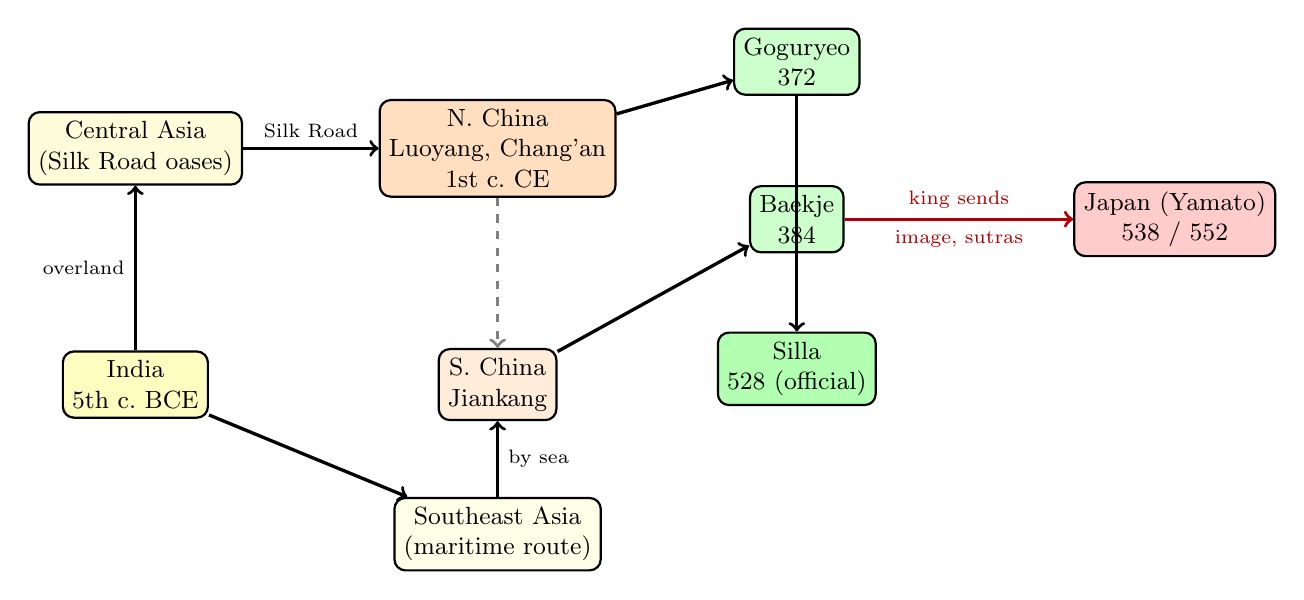
\begin{tikzpicture}[x=1cm, y=1cm,
    pl/.style={draw, thick, rounded corners, align=center, font=\small, fill=white},
    ar/.style={->, very thick}]
  \node[pl, fill=yellow!25] (ind) at (-6.6,-1.5) {India\\5th c.\ BCE};
  \node[pl, fill=yellow!15] (ca) at (-6.6,1.5) {Central Asia\\(Silk Road oases)};
  \node[pl, fill=orange!25] (lo) at (-2,1.5) {N.\ China\\Luoyang, Chang'an\\1st c.\ CE};
  \node[pl, fill=orange!15] (sc) at (-2,-1.5) {S.\ China\\Jiankang};
  \node[pl, fill=green!20] (gog) at (1.8,2.6) {Goguryeo\\372};
  \node[pl, fill=green!20] (bae) at (1.8,0.6) {Baekje\\384};
  \node[pl, fill=green!30] (sil) at (1.8,-1.3) {Silla\\528 (official)};
  \node[pl, fill=red!20] (jp) at (6.6,0.6) {Japan (Yamato)\\538 / 552};
  \node[pl, fill=yellow!10] (sea) at (-2,-3.4) {Southeast Asia\\(maritime route)};
  \draw[ar] (ind) -- node[left, font=\scriptsize] {overland} (ca);
  \draw[ar] (ca) -- node[above, font=\scriptsize] {Silk Road} (lo);
  \draw[ar] (ind) -- (sea);
  \draw[ar] (sea) -- node[right, font=\scriptsize] {by sea} (sc);
  \draw[ar] (lo) -- (gog);
  \draw[ar] (sc) -- (bae);
  \draw[ar] (gog) -- (sil);
  \draw[ar, red!70!black] (bae) -- node[above, font=\scriptsize] {king sends} node[below, font=\scriptsize] {image, sutras} (jp);
  \draw[ar, dashed, gray] (lo) -- (sc);
\end{tikzpicture}
\end{center}

\begin{important}[Dates to know]
\begin{itemize}
  \item c.\ 1st century CE: Buddhism reaches China via Central Asian merchants and monks.
  \item 372: a Former Qin monk brings images and sutras to Goguryeo.
  \item 384: Baekje receives the Serindian monk Marananta.
  \item 527/528: Silla adopts Buddhism officially after the martyrdom of Ichadon.
  \item 538 (or 552): the Baekje king sends an image and sutras to the Yamato court.
\end{itemize}
\end{important}

\section{Sinicization: making Buddhism Chinese}

Buddhism faced serious obstacles in China:

\begin{center}
\begin{tabular}{p{5.5cm}p{7.5cm}}
\toprule
Objection & Buddhist response \\
\midrule
Monks leave their families and do not produce heirs: unfilial. & Monks earn merit that
benefits ancestors; sutras on filial piety (some composed in China); the Ghost Festival
rescues parents from hell (the story of Mulian). \\
Monks do not bow to the emperor and do not pay taxes. & Long debates (Huiyuan, 4th c.);
eventually the state registered and controlled the clergy. \\
It is foreign (``barbarian'') teaching. & Translation into Chinese terms, sometimes using
Daoist vocabulary (``matching concepts''); legend that Laozi went west and taught the
Buddha. \\
\bottomrule
\end{tabular}
\end{center}

\subsection{Translation}

Translators such as \textbf{Kumārajīva} (344--413), a Central Asian monk brought to
Chang'an, produced fluent Chinese versions of key sutras (\emph{Lotus Sutra},
\emph{Diamond Sutra}). The pilgrim \textbf{Xuanzang} (602--664) travelled to India for
seventeen years and returned with hundreds of texts; his journey became the basis of the
Ming novel \emph{Journey to the West} (with the Monkey King, Sun Wukong).

\subsection{Chinese schools}

\begin{center}
\begin{tabular}{llll}
\toprule
School & China & Korea & Japan \\
\midrule
Tiantai (Lotus Sutra) & \zht{天台} Tiāntái & Cheontae \ko{천태} & Tendai \ja{天台} \\
Huayan (Flower Garland) & \zht{華嚴} Huáyán & Hwaeom \ko{화엄} & Kegon \ja{華厳} \\
Pure Land (Amitābha) & \zht{淨土} Jìngtǔ & Jeongto \ko{정토} & Jōdo \ja{浄土} \\
Meditation & \zht{禪} Chán & Seon \ko{선} & Zen \ja{禅} \\
Esoteric (mantras, mandalas) & \zht{密宗} Mìzōng & Milgyo \ko{밀교} & Shingon \ja{真言} \\
\bottomrule
\end{tabular}
\end{center}

\section{Chan / Seon / Zen}

\begin{definition}[Chan]
\emph{Chan} (from Sanskrit \emph{dhyāna}, ``meditation'') is a school claiming a
``separate transmission outside the scriptures'', from mind to mind, beginning when the
Buddha silently held up a flower and his disciple Mahākāśyapa smiled. Its legendary
founder in China is the Indian monk Bodhidharma (c.\ 5th--6th c.).
\end{definition}

\begin{itemize}
  \item \textbf{Sudden vs.\ gradual enlightenment}: the Sixth Patriarch Huineng (638--713),
        an illiterate kitchen worker in the \emph{Platform Sutra} story, wins the
        succession with a poem asserting that the mind is originally pure, so awakening is
        sudden.
  \item \textbf{Gong'an / kōan} (\zht{公案}): paradoxical exchanges (``What is the sound of
        one hand?'', the ``Mu'' kōan) used to break through conceptual thinking.
  \item \textbf{Korea}: Seon arrived in the 8th--9th centuries (``Nine Mountain'' schools).
        Jinul (1158--1210) combined Seon practice with doctrinal study; the Jogye Order is
        the largest Korean Buddhist order today.
  \item \textbf{Japan}: Eisai brought Rinzai Zen (1191), favoured by the Kamakura and
        Muromachi shogunates; Dōgen brought Sōtō Zen (1227), emphasizing ``just sitting''
        (\ja{只管打坐}, shikantaza).
\end{itemize}

\begin{aside}
Zen in the West (D.\,T.\ Suzuki, the 1950s ``Beat Zen'') was presented as a timeless,
anti-institutional mysticism. Historically, Zen in Japan was a powerful institution closely
tied to warrior rulers, to the arts (ink painting, tea, gardens) and, in the 20th century,
to nationalism. A good example of how a tradition is re-imagined as it travels.
\end{aside}

\section{Buddhism and the state}

\begin{itemize}
  \item \textbf{China}: emperors patronized Buddhism (Empress Wu Zetian presented herself
        as a future Buddha), but the Tang \textbf{Huichang persecution} (842--845)
        destroyed thousands of monasteries and laicized some 260\,000 monks and nuns,
        largely for fiscal reasons. Buddhism survived, but Chan and Pure Land (which needed
        fewer texts and institutions) did best afterwards.
  \item \textbf{Korea}: ``state-protection Buddhism''. Silla and Goryeo were strongly
        Buddhist. Goryeo carved the entire canon on over 80\,000 woodblocks (the
        \emph{Tripitaka Koreana}, 13th c., still at Haeinsa temple) to win divine
        protection against the Mongols. Joseon then suppressed Buddhism in favour of
        Neo-Confucianism, pushing monasteries into the mountains.
  \item \textbf{Japan}: Prince Shōtoku (574--622) is remembered as a great patron
        (Hōryūji temple). Emperor Shōmu built Tōdaiji and its Great Buddha (752) and a
        network of provincial temples. In the Kamakura period new popular schools appeared:
        Pure Land (Hōnen, Shinran), Nichiren (Lotus Sutra devotion) and Zen.
\end{itemize}

\begin{center}
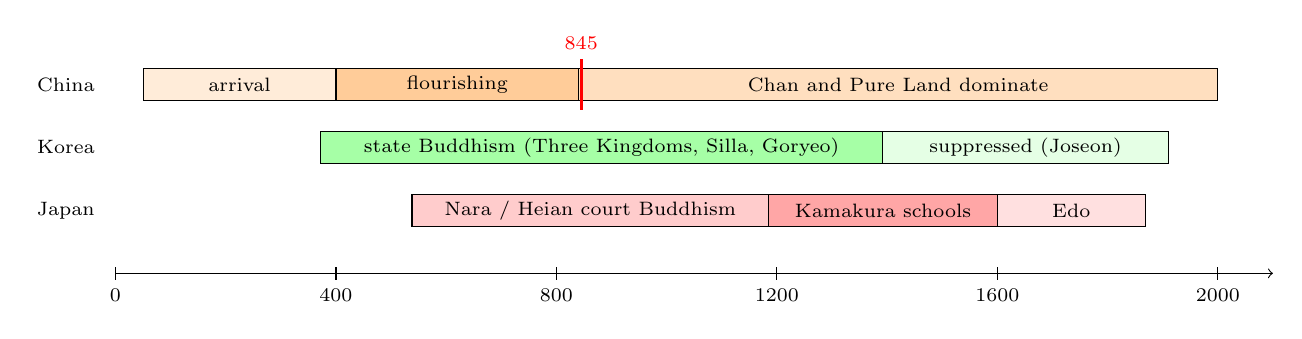
\begin{tikzpicture}[x=0.7cm, y=0.8cm, every node/.style={font=\scriptsize}]
  \draw[->] (0,0) -- (21,0);
  \foreach \x/\l in {0/0, 4/400, 8/800, 12/1200, 16/1600, 20/2000} {
    \draw (\x,0.1) -- (\x,-0.1) node[below] {\l};
  }
  % China
  \node[anchor=east] at (-0.2,3) {China};
  \draw[fill=orange!15] (0.5,2.75) rectangle (4,3.25) node[midway] {arrival};
  \draw[fill=orange!40] (4,2.75) rectangle (8.4,3.25) node[midway] {flourishing};
  \draw[fill=orange!25] (8.4,2.75) rectangle (20,3.25) node[midway] {Chan and Pure Land dominate};
  \draw[very thick, red] (8.45,2.6) -- (8.45,3.4);
  \node[red, above] at (8.45,3.4) {845};
  % Korea
  \node[anchor=east] at (-0.2,2) {Korea};
  \draw[fill=green!35] (3.72,1.75) rectangle (13.92,2.25) node[midway] {state Buddhism (Three Kingdoms, Silla, Goryeo)};
  \draw[fill=green!10] (13.92,1.75) rectangle (19.1,2.25) node[midway] {suppressed (Joseon)};
  % Japan
  \node[anchor=east] at (-0.2,1) {Japan};
  \draw[fill=red!20] (5.38,0.75) rectangle (11.85,1.25) node[midway] {Nara / Heian court Buddhism};
  \draw[fill=red!35] (11.85,0.75) rectangle (16,1.25) node[midway] {Kamakura schools};
  \draw[fill=red!12] (16,0.75) rectangle (18.68,1.25) node[midway] {Edo};
\end{tikzpicture}
\end{center}

\begin{remark}
In the Edo period every Japanese household had to register with a Buddhist temple (the
\emph{danka} system) to prove it was not Christian. This is why funerals in Japan are still
mostly Buddhist (``Shinto for life events, Buddhism for death'').
\end{remark}

\section{Buddhism and material culture}

\begin{itemize}
  \item \textbf{Printing}: the oldest dated printed book is a Chinese \emph{Diamond Sutra}
        (868), found at Dunhuang; a Korean dhāraṇī scroll (before 751) may be older. Korea's
        \emph{Jikji} (1377) is the oldest extant book printed with movable metal type.
  \item \textbf{Architecture}: pagodas (from the Indian stupa), cave temples (Dunhuang,
        Longmen, Seokguram in Korea).
  \item \textbf{Tea}: spread with Chan/Zen monks as an aid to meditation.
\end{itemize}

\section*{Summary}
\begin{itemize}
  \item Mahayana Buddhism came from India via Central Asia (and the sea) to China, then to
        Korea (4th c.) and from Baekje to Japan (6th c.).
  \item It was sinicized to answer objections (filial piety, the state, foreignness).
  \item Major schools have names in all three languages: Chan/Seon/Zen, Pure
        Land, Tiantai/Tendai, Huayan/Kegon.
  \item Fortunes differed: persecuted in Tang China, suppressed in Joseon Korea,
        institutionally entrenched in Japan.
  \item Buddhism drove printing, architecture and tea culture across the region.
\end{itemize}
